Jméno: \hspace{4cm} Login: \hspace{4cm} Skupina cvičení:\\
Datum:

\section{Komunikace VoIP type peer-to-peer}
\begin{multicols}{2}
  \begin{center}
    
\includegraphics[width=70mm]{peer-to-peer.eps}
  \end{center}
  \columnbreak
  \subsection*{Klient A}      
  \begin{enumerate}
    \item Signalizace SIP
    
    \begin{tabular}{lp{2cm}}
      IP adresa a port stanice A: &\\
      IP adresa a port stanice B: &\\
    \end{tabular}               
   
    \item Transport hlasových dat RTP
    
    \begin{tabular}{lp{2cm}}
      IP adresa a port stanice A: &\\
      IP adresa a port stanice B: &\\
      Seznam podporovaných kodeků (pouze čísla):&\\
      &\\
      Použitý kodek (název a číslo): &\\
    \end{tabular}               
  \end{enumerate}      
\end{multicols}

\section{Registrace klient VoIP na ústředně}
\begin{multicols}{2}
  \begin{center}
    
\includegraphics[width=70mm]{registrace.eps}
  \end{center}
    Čím se liší obsah paketu REGISTER při odhlášení od paketu při přihlášení?
  \columnbreak
  
  \begin{tabular}{lp{2cm}}
    &\\
    IP adresa a port serveru: &\\
    Název a verze sw serveru: &\\
    &\\
    &\\
    User URI klienta: &\\
    Device URI klienta: &\\
    &\\
    Název a verze sw klienta: &\\
    &\\
    Max. doba přihlášení: &\\
  \end{tabular}               
\end{multicols}

\section{Komunikace VoIP přes ústřednu (z pohledu volajícího)}
  \begin{center}    
    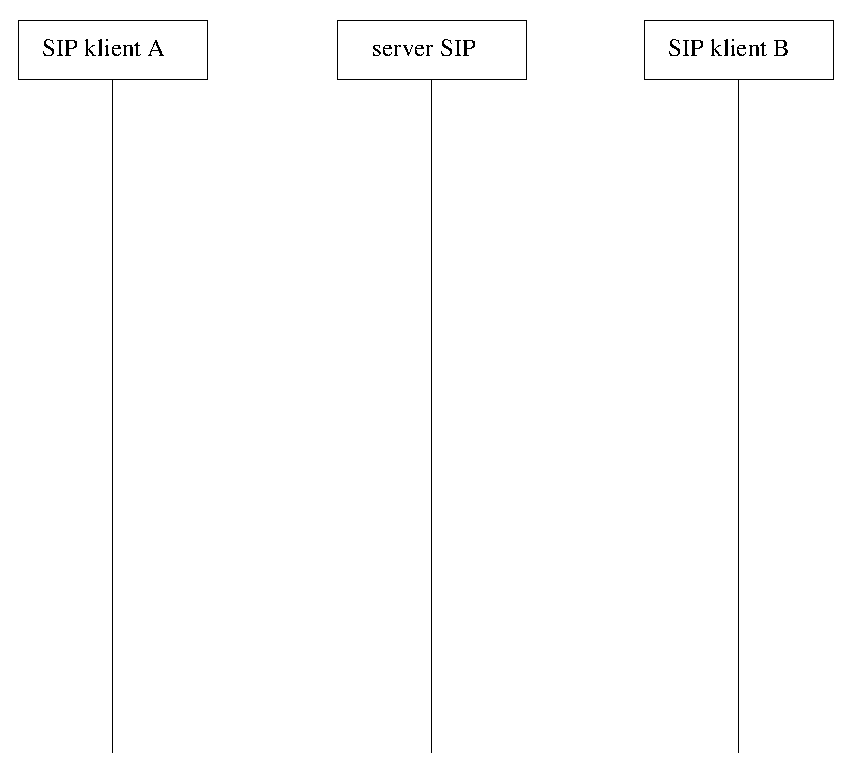
\includegraphics[width=120mm]{pres-ustrednu.eps}
  \end{center}
  \vspace{1cm}

  \subsection*{A) Signalizace}
  \begin{tabular}{lp{2cm}}
    IP adresa a port volající stanice A: &\\
    IP adresa a port serveru: &\\
    &\\
    User URI volajícího: &\\
    Device URI volajícího: &\\
    &\\
    User URI volaného: &\\
    Device URI volaného: &\\
  \end{tabular}               

  \subsection*{B) Transport hlasových dat}
  \begin{tabular}{lp{2cm}}
    IP adresa a port RTP volající stanice A: &\\
    &\\
    IP adresa a port RTP volané stanice B: &\\
    &\\
    Vybraný kodek (název a číslo): &\\
    &\\
    Počet přenesených paketů RTP (A $\rightarrow$ B): &\\
    &\\
    Počet přenesených paketů RTP (B $\rightarrow$ A): &\\
\end{tabular}               
